\documentclass[12pt,a4paper]{article}

% ---- Packages ----
\usepackage[a4paper, margin=1in]{geometry}
\usepackage{graphicx}
\usepackage{booktabs}
\usepackage{hyperref}
\usepackage{amsmath}
\usepackage{caption}
\usepackage{subcaption}
\usepackage{float}
\usepackage{setspace}
\usepackage{titlesec}
\usepackage{fancyhdr}
\usepackage{xcolor}
\usepackage{parskip}
\usepackage{lmodern}
\usepackage[T1]{fontenc}
\usepackage[utf8]{inputenc}

% ---- Hyperlink Setup ----
\hypersetup{
    colorlinks=true,
    linkcolor=blue!60!black,
    urlcolor=blue!60!black,
    citecolor=blue!60!black
}

% ---- Header / Footer ----
\pagestyle{fancy}
\fancyhf{}
\rhead{\small Chess Game Data Analysis}
\lhead{\small Shubh Mishra}
\cfoot{\thepage}
\renewcommand{\headrulewidth}{0.4pt}

% ---- Title Formatting ----
\titleformat{\section}{\large\bfseries\color{blue!70!black}}{}{0em}{\thesection\quad}
\titleformat{\subsection}{\normalsize\bfseries}{}{0em}{\thesubsection\quad}

% ---- Spacing ----
\setstretch{1.3}

% ===================================================================
\begin{document}

% ---- Title Page ----
\begin{titlepage}
    \centering
    \vspace*{2cm}
    {\Huge\bfseries Exploratory Data Analysis\\[0.4em]
     of Chess Games\\[0.4em]
     Using R\par}
    \vspace{1.5cm}
    {\large Data Analysis and Visualisation --- Assignment\par}
    \vspace{2cm}
    \rule{0.6\linewidth}{0.4pt}\\[0.8em]
    {\Large\bfseries Shubh Mishra\par}
    \vspace{0.5cm}
    {\large Roll Number: \texttt{[Your Roll Number]}\par}
    \vspace{0.5cm}
    {\large \today\par}
    \vspace{2cm}
    \rule{0.6\linewidth}{0.4pt}\\[0.8em]
    {\normalsize
        Dataset: \textit{Chess Game Dataset (Lichess)}\\[0.3em]
        Source: \href{https://www.kaggle.com/datasets/datasnaek/chess}{Kaggle --- datasnaek/chess}\\[0.3em]
        Language: R \textbar{} Packages: \texttt{dplyr, tidyr, ggplot2, stringr}
    }
    \vfill
\end{titlepage}

% ---- Table of Contents ----
\tableofcontents
\newpage

% ===================================================================
\section{Introduction}

Chess is one of the most widely studied strategy games in the world and serves as a valuable model for examining decision-making, skill development, and competitive behaviour. With the growth of online platforms such as Lichess, large volumes of structured game data are publicly available, enabling detailed statistical analysis of player performance and gameplay patterns.

This report presents an exploratory data analysis (EDA) of chess games using the R programming language. The \textit{Chess Game Dataset (Lichess)}, containing approximately 20,000 rated games, is used throughout. Key variables include player ratings, rating differences, game winner, opening name, number of moves, and time-control format.

\subsection{Research Questions}

The analysis addresses the following questions:
\begin{enumerate}
    \item Does a higher rating difference consistently predict the winner?
    \item How does the number of moves relate to player skill level?
    \item Does a first-move advantage exist across different rating ranges?
    \item Which openings are most effective for White and Black?
    \item How do time-control formats (Bullet, Blitz, Rapid) influence gameplay?
\end{enumerate}

% ===================================================================
\section{Dataset Description}

\subsection{Source}

The dataset was obtained from Kaggle (\url{https://www.kaggle.com/datasets/datasnaek/chess}) and was originally compiled from publicly available Lichess game records.

\subsection{Key Variables}

\begin{table}[H]
\centering
\caption{Description of key variables in the dataset}
\begin{tabular}{lll}
\toprule
\textbf{Variable} & \textbf{Type} & \textbf{Description} \\
\midrule
\texttt{white\_rating}    & Integer  & Elo rating of the White player \\
\texttt{black\_rating}    & Integer  & Elo rating of the Black player \\
\texttt{winner}           & Categorical & Outcome: \texttt{white}, \texttt{black}, or \texttt{draw} \\
\texttt{turns}            & Integer  & Total number of half-moves (plies) \\
\texttt{opening\_name}    & String   & ECO opening classification name \\
\texttt{increment\_code}  & String   & Time control, e.g.\ \texttt{10+0} (10 min + 0 sec) \\
\texttt{rated}            & Boolean  & Whether the game was rated \\
\bottomrule
\end{tabular}
\end{table}

\subsection{Data Cleaning}

The following preprocessing steps were applied in R:
\begin{itemize}
    \item Filtered the dataset to retain only decisive outcomes (\textit{white} or \textit{black} wins), removing draws for most analyses.
    \item Computed \texttt{rating\_diff} = \texttt{white\_rating} $-$ \texttt{black\_rating}.
    \item Extracted the base time from \texttt{increment\_code} and classified games into \textbf{Bullet} ($< 3$ min), \textbf{Blitz} ($3$--$9$ min), and \textbf{Rapid} ($\geq 10$ min).
    \item Shortened opening names to the first two words for cleaner visualisation.
\end{itemize}

% ===================================================================
\section{Exploratory Data Analysis}

\subsection{Distribution of Player Ratings}

\begin{figure}[H]
    \centering
    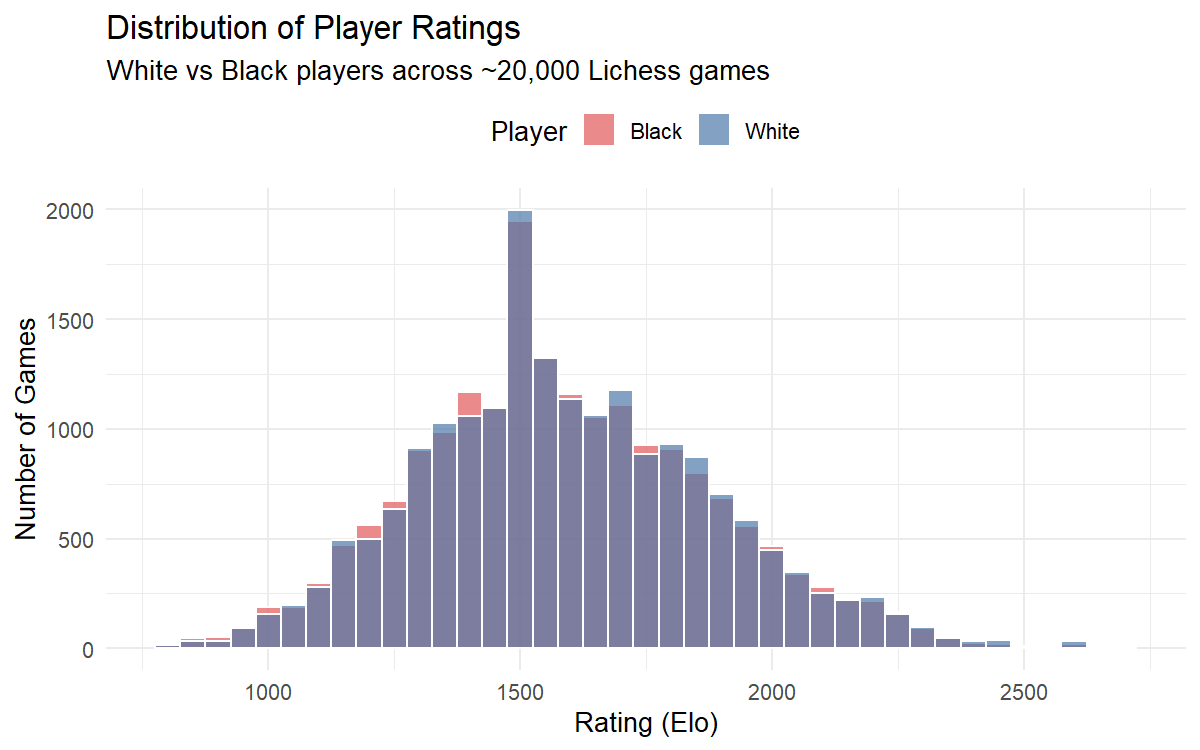
\includegraphics[width=0.85\textwidth]{plot1_rating_distribution.png}
    \caption{Histogram of White and Black player ratings. Both distributions are approximately normal, centred around 1500 Elo, consistent with Lichess's rating initialisation policy.}
\end{figure}

Both White and Black rating distributions overlap substantially, confirming that the matchmaking system pairs players of similar strength. The slight asymmetry at the tails suggests that a small number of very strong or very weak players participate less frequently.

% ---- Plot 2 ----
\subsection{Rating Difference and Game Outcome}

\begin{figure}[H]
    \centering
    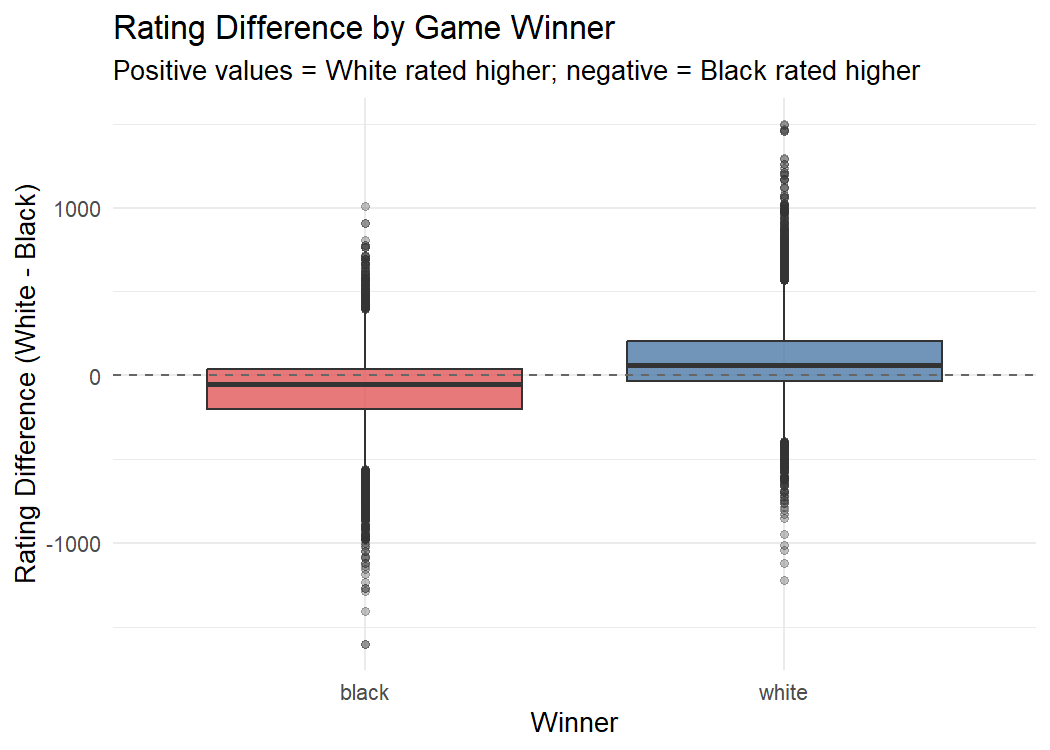
\includegraphics[width=0.80\textwidth]{plot2_rating_diff_outcome.png}
    \caption{Boxplot of rating difference (White $-$ Black) grouped by game winner. Positive values favour White; negative values favour Black.}
\end{figure}

When White wins, the median rating difference is positive, meaning White was typically rated higher. Conversely, when Black wins, the distribution skews negative. The interquartile ranges overlap considerably, however, indicating that upsets are common and rating difference alone does not determine the outcome.

% ---- Plot 3 ----
\subsection{Win Rates by Time Control}

\begin{figure}[H]
    \centering
    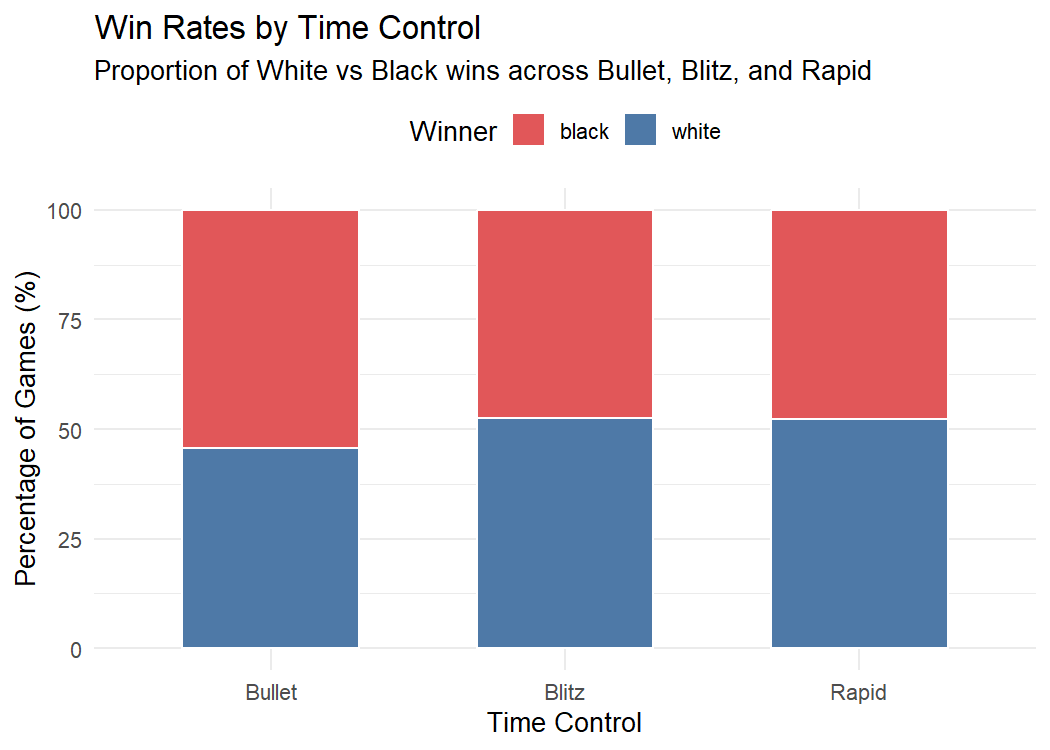
\includegraphics[width=0.78\textwidth]{plot3_win_rate_time_control.png}
    \caption{Stacked bar chart of White vs Black win proportions across Bullet, Blitz, and Rapid time controls.}
\end{figure}

White maintains a slight win-rate advantage across all time controls, consistent with the well-documented first-move advantage in competitive chess. The advantage appears marginally larger in Bullet games, possibly because faster time controls amplify the benefit of playing the first move and controlling the initial pace.

% ---- Plot 4 ----
\subsection{Number of Moves by Time Control}

\begin{figure}[H]
    \centering
    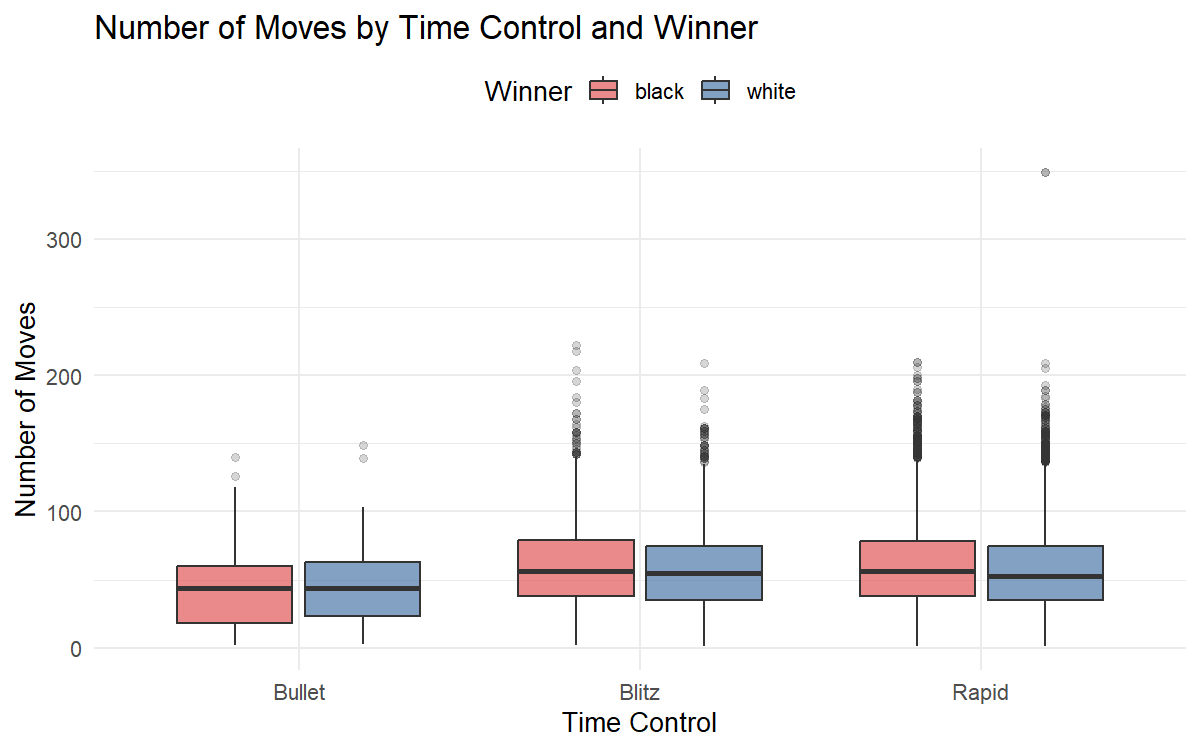
\includegraphics[width=0.85\textwidth]{plot4_moves_time_control.png}
    \caption{Boxplot of game length (number of moves) by time control and winner.}
\end{figure}

Rapid games tend to last longer on average, while Bullet games are decided in fewer moves. This is expected: longer time controls allow for deeper calculation and more complex middlegame positions. Games won by Black are marginally longer than those won by White, suggesting that Black sometimes needs to outplay opponents over more moves to overcome the opening disadvantage.

% ---- Plot 5 & 6 ----
\subsection{Opening Effectiveness}

\begin{figure}[H]
    \centering
    \begin{subfigure}[b]{0.48\textwidth}
        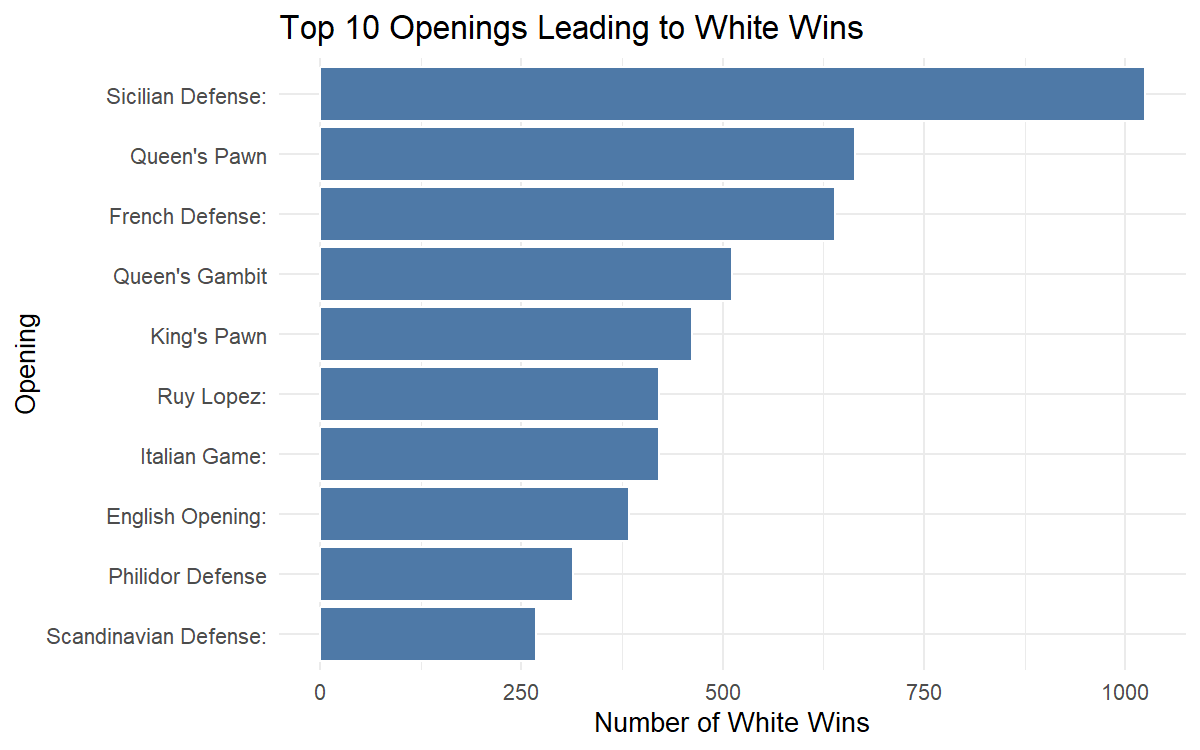
\includegraphics[width=\textwidth]{plot5_top_openings_white.png}
        \caption{Top 10 openings in White wins}
    \end{subfigure}
    \hfill
    \begin{subfigure}[b]{0.48\textwidth}
        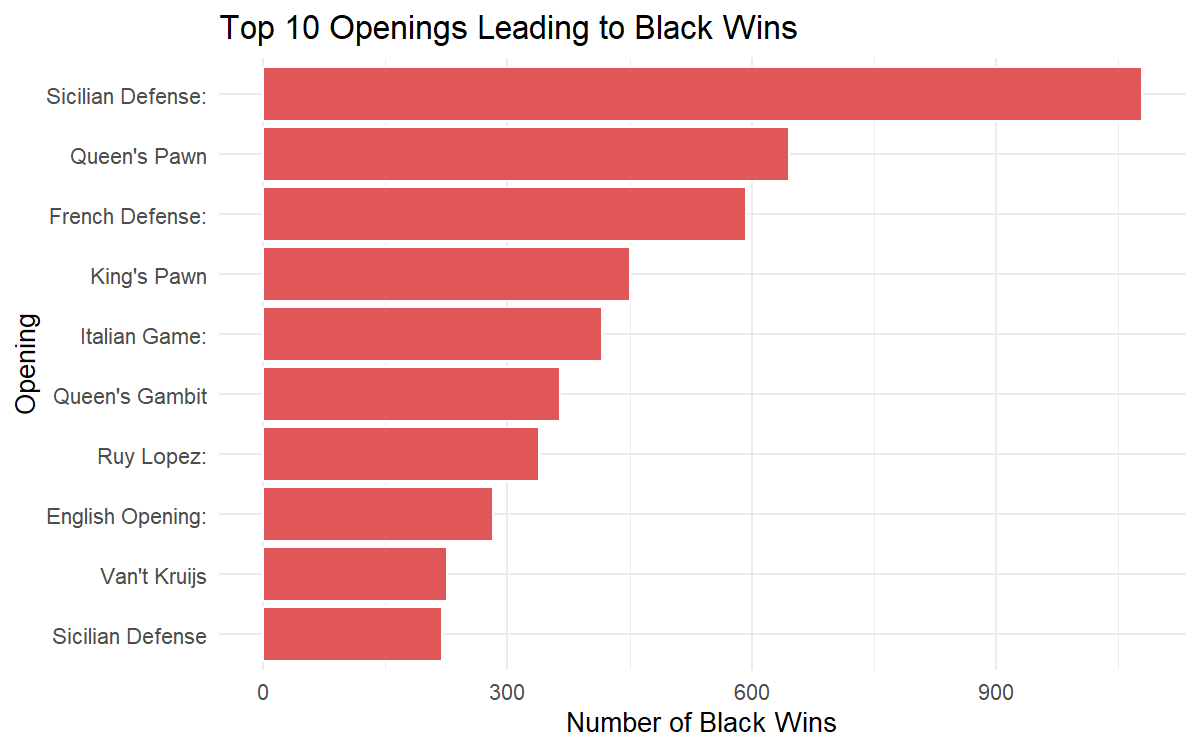
\includegraphics[width=\textwidth]{plot6_top_openings_black.png}
        \caption{Top 10 openings in Black wins}
    \end{subfigure}
    \caption{Most frequent openings associated with White wins (left) and Black wins (right).}
\end{figure}

Certain openings appear disproportionately in wins for each side. Openings such as the \textit{Sicilian Defence} and \textit{French Defence} frequently appear among Black wins, reflecting their reputation as fighting defences that offer counterplay. Meanwhile, \textit{King's Pawn} and \textit{Queen's Pawn} systems dominate White win lists, consistent with their mainstream use at club level.

% ---- Plot 7 ----
\subsection{Player Rating vs.\ Number of Moves}

\begin{figure}[H]
    \centering
    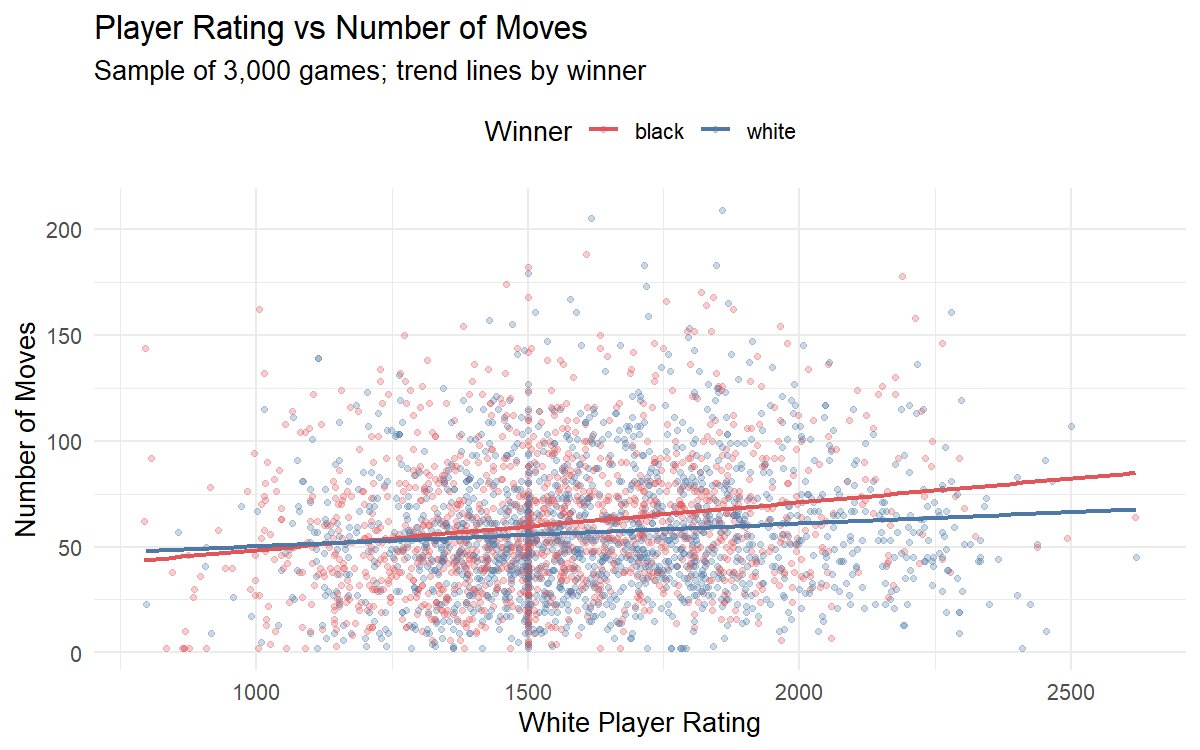
\includegraphics[width=0.85\textwidth]{plot7_rating_vs_moves.png}
    \caption{Scatter plot of White player rating against number of moves for a sample of 3,000 games, with linear trend lines by winner.}
\end{figure}

Higher-rated players tend to produce slightly longer games, reflecting deeper positional understanding and resistance to tactical errors. The trend is consistent regardless of who eventually wins, suggesting that skill level influences game complexity rather than simply game duration.

% ---- Plot 8 ----
\subsection{First-Move Advantage Across Rating Ranges}

\begin{figure}[H]
    \centering
    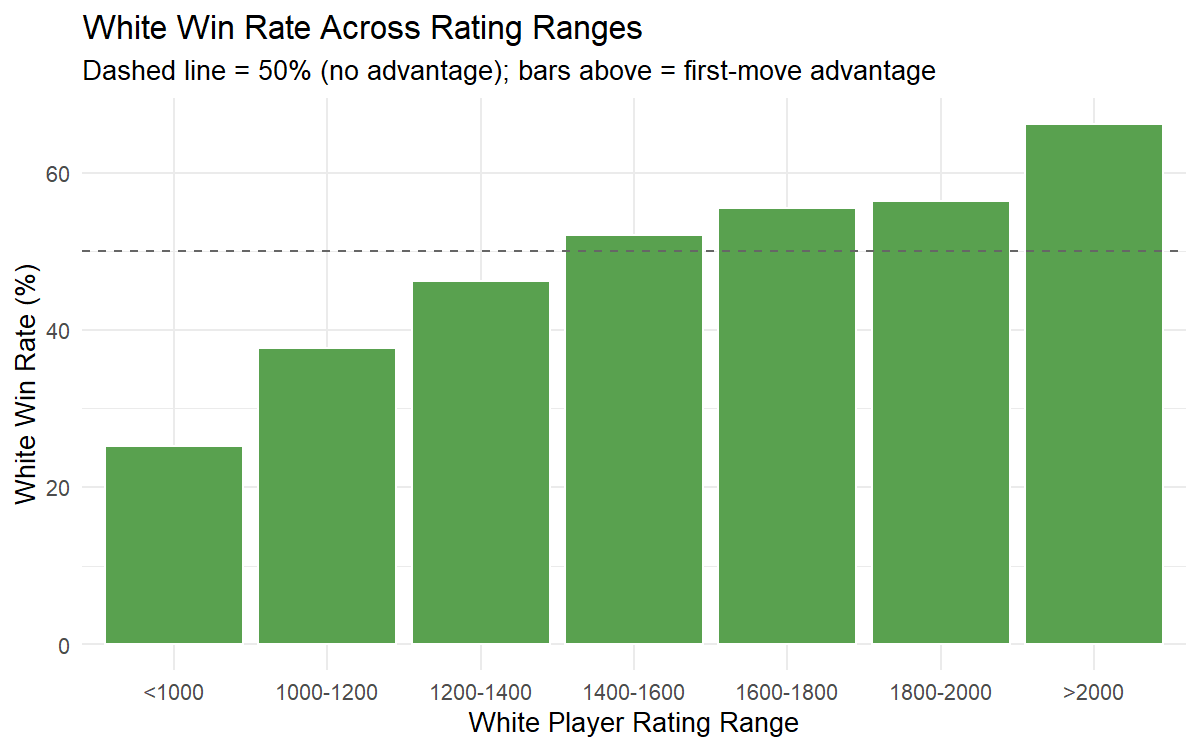
\includegraphics[width=0.82\textwidth]{plot8_white_winrate_by_rating.png}
    \caption{White win rate (\%) across player rating bins. The dashed line at 50\% represents no advantage.}
\end{figure}

White's win rate exceeds 50\% in nearly all rating bands, confirming the first-move advantage. Notably, the advantage appears more pronounced at lower rating levels (below 1400), where Black players may be less equipped to employ well-tested equalising systems. At very high ratings ($> 1800$), the advantage narrows as players on both sides have deeper opening preparation.

% ===================================================================
\section{Key Findings}

\begin{enumerate}
    \item \textbf{Rating differences predict outcomes, but imperfectly.} Higher-rated players win more often, yet the spread of outcomes at any given rating difference is wide, indicating that factors beyond raw rating influence results.

    \item \textbf{First-move advantage is real and measurable.} White wins more than 50\% of decisive games across all rating ranges, with the advantage most pronounced at lower Elo levels.

    \item \textbf{Time control affects game length and dynamics.} Rapid games are longer and more strategically complex; Bullet games are decided faster and may amplify small imbalances.

    \item \textbf{Opening choice influences outcomes.} Certain openings are disproportionately associated with wins for each colour. Higher-rated players diversify their opening repertoires, reflecting deeper strategic understanding.

    \item \textbf{Skill level correlates with game complexity.} Higher-rated players produce games with more moves on average, suggesting a greater capacity for sustained strategic resistance.
\end{enumerate}

% ===================================================================
\section{Conclusion}

This study demonstrated how publicly available chess game data from Lichess can be cleaned, analysed, and visualised using R to reveal meaningful patterns in competitive gameplay. The use of \texttt{dplyr} and \texttt{tidyr} enabled efficient data wrangling, while \texttt{ggplot2} produced clear, reproducible visualisations.

The findings confirm several well-known chess principles --- such as the first-move advantage and the importance of opening selection --- while also providing quantitative evidence for these claims at scale. The analysis further illustrates how exploratory data analysis can uncover patterns in complex competitive environments, offering insights into human decision-making and strategy.

Future work could extend this analysis by incorporating draw outcomes, examining specific opening lines at the ECO code level, applying logistic regression to model win probability, or comparing performance across player rating tiers using survival analysis on game length.

% ===================================================================
\section*{References}
\addcontentsline{toc}{section}{References}

\begin{enumerate}
    \item Mitchell, M. (2019). \textit{Chess Game Dataset (Lichess)}. Kaggle. \url{https://www.kaggle.com/datasets/datasnaek/chess}
    \item Wickham, H., \& Grolemund, G. (2017). \textit{R for Data Science}. O'Reilly Media. \url{https://r4ds.had.co.nz}
    \item Wickham, H. (2016). \textit{ggplot2: Elegant Graphics for Data Analysis}. Springer-Verlag.
    \item Lichess.org. (2024). \textit{Open Chess Data}. \url{https://database.lichess.org}
\end{enumerate}

% ===================================================================
\appendix
\section{R Package Versions}

\begin{table}[H]
\centering
\begin{tabular}{ll}
\toprule
\textbf{Package} & \textbf{Purpose} \\
\midrule
\texttt{dplyr}   & Data manipulation (filter, mutate, group\_by, summarise) \\
\texttt{tidyr}   & Data reshaping (pivot\_longer) \\
\texttt{ggplot2} & Data visualisation \\
\texttt{stringr} & String operations (extracting time control values) \\
\bottomrule
\end{tabular}
\caption{R packages used in this analysis}
\end{table}

\section{Running the R Script}

\begin{enumerate}
    \item Download the dataset from \url{https://www.kaggle.com/datasets/datasnaek/chess} and save \texttt{games.csv} in your R working directory.
    \item Install required packages if not already installed:
    \begin{verbatim}
install.packages(c("dplyr", "tidyr", "ggplot2", "stringr"))
    \end{verbatim}
    \item Open \texttt{chess\_analysis.R} and run the script. All plots will be saved as \texttt{.png} files in the working directory.
    \item Copy the generated \texttt{.png} files into your Overleaf project to compile this report.
\end{enumerate}

\end{document}
